\documentclass[12pt]{scrartcl}

\usepackage[T1]{fontenc}
\usepackage[utf8]{inputenc}
\usepackage{amsmath}
\usepackage{amsfonts}
\usepackage{amssymb}
\usepackage{amsbsy}
\usepackage{graphicx}
\usepackage{float}
\usepackage{array}
\usepackage{booktabs}
\usepackage{multirow}
\usepackage{bm}
\usepackage{verbatim}
\usepackage[english]{babel}
\usepackage{color}
\usepackage{url}
\usepackage{fancybox}
\usepackage[stable]{footmisc}
\usepackage[format=plain,labelfont=bf]{caption}
\usepackage{fancyhdr}
\usepackage{natbib}
\usepackage{calc}
\usepackage{textcomp}
\usepackage[pdftex,pdfborder={0 0 0}]{hyperref}
\usepackage{pdfpages}
\usepackage{tikz}
\usetikzlibrary{shapes,backgrounds,fit,positioning,arrows,positioning,decorations.pathmorphing,decorations.pathreplacing,backgrounds}
\usepackage{accents}

\renewcommand*{\familydefault}{\sfdefault}

% Margins
\addtolength{\textheight}{1.0cm}
\addtolength{\oddsidemargin}{-0.5cm}
\addtolength{\evensidemargin}{-0.5cm}
\addtolength{\textwidth}{1.0cm}
\parindent=0em

% Appropriate font for \mathcal{}
\DeclareSymbolFont{cmmathcal}{OMS}{cmsy}{m}{n}
\DeclareSymbolFontAlphabet{\mathcal}{cmmathcal}

% Set subscript and superscripts positions
\everymath{
\fontdimen13\textfont2=5pt
\fontdimen14\textfont2=5pt
\fontdimen15\textfont2=5pt
\fontdimen16\textfont2=5pt
\fontdimen17\textfont2=5pt
}

% Bibliography style
\setlength{\bibsep}{1pt}

% Part
\renewcommand\partheadstartvskip{\clearpage\null\vfil}
\renewcommand\partheadmidvskip{\par\nobreak\vskip 20pt\thispagestyle{empty}}
\renewcommand\partheadendvskip{\vfil\clearpage}
\renewcommand\raggedpart{\centering}

\begin{document}
\title{Bi-Fourier spectral B matrix}
\author{Benjamin Ménétrier}
\date{Last update: \today}

\thispagestyle{empty}

\maketitle

\tableofcontents

\clearpage

\section*{Introduction}

This documents describes the \texttt{Bifourier} blocks implemented in the SABER library to apply a static background error covariance matrix in spectral space. The code is a generalization of the implementation of \cite{berre_2000}.

\section{Spectral transform}

This section details the spectral transform characteristics.

\subsection{Parallelization}

The spectral transform process starts with a field of size $n_x \times n_y$ in physical space, split among several MPI tasks. For instance:

\begin{center}
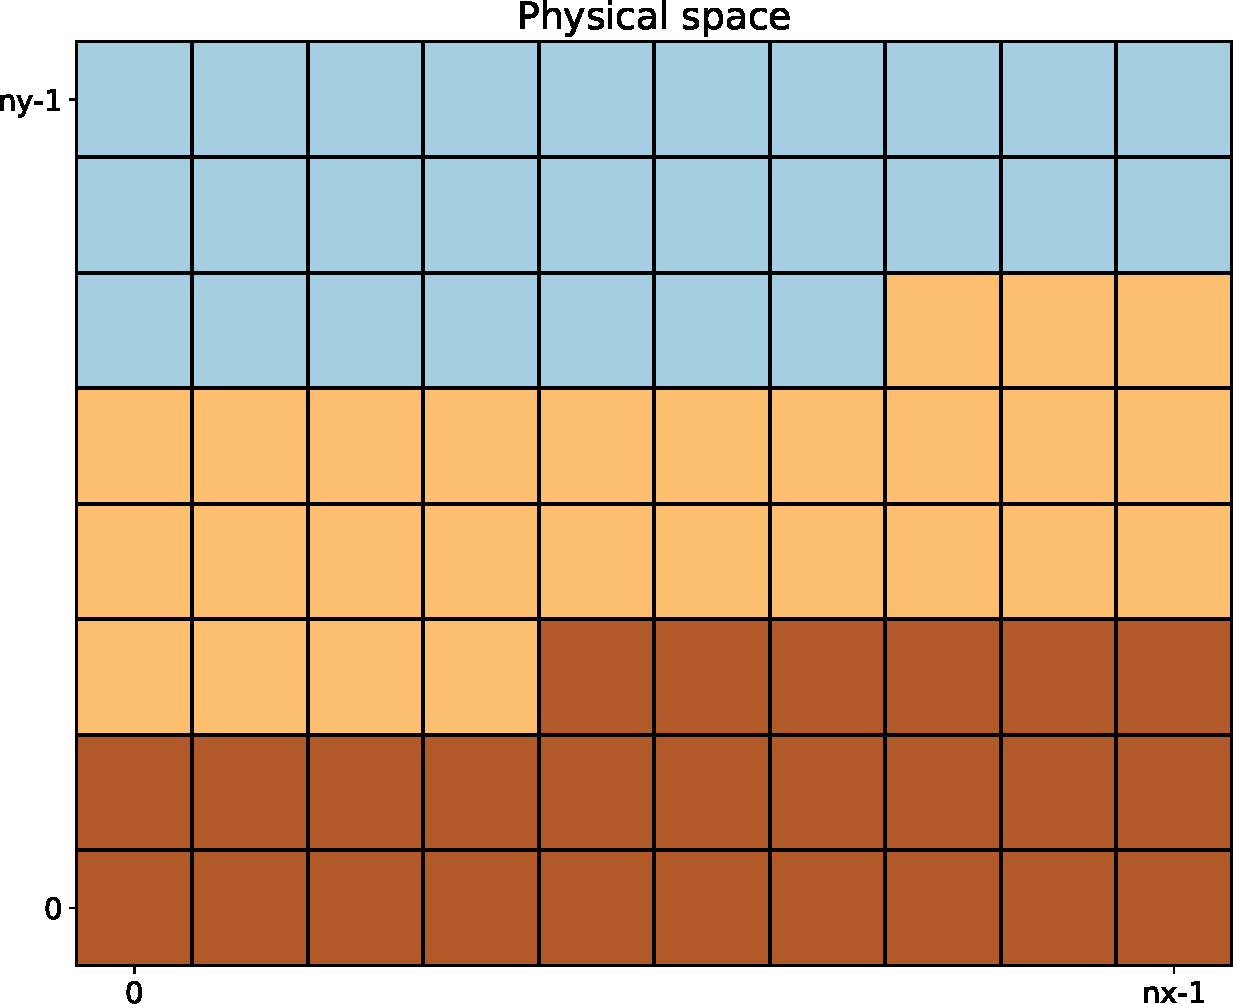
\includegraphics[width=0.5\textwidth]{step0.pdf}
\end{center}

The first step is a global communication (\texttt{MPI\_Alltoallv}) to make sure that each row is handled by a single task:

\begin{center}
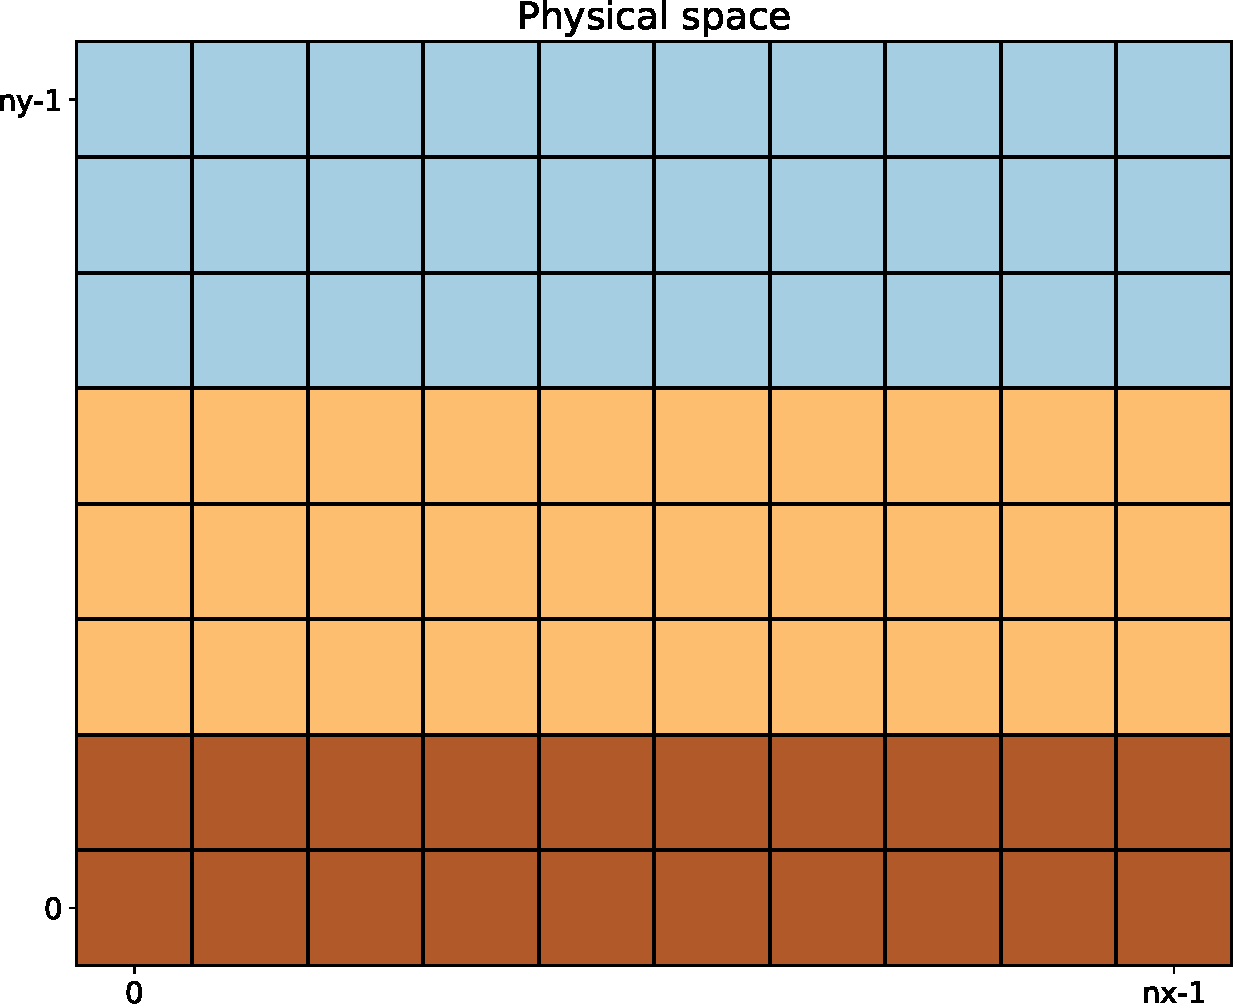
\includegraphics[width=0.5\textwidth]{step1.pdf}
\end{center}

The second step is a FFT along each row, leading to two arrays of size $n_k \times n_y$ for real and imaginary components:

\begin{center}
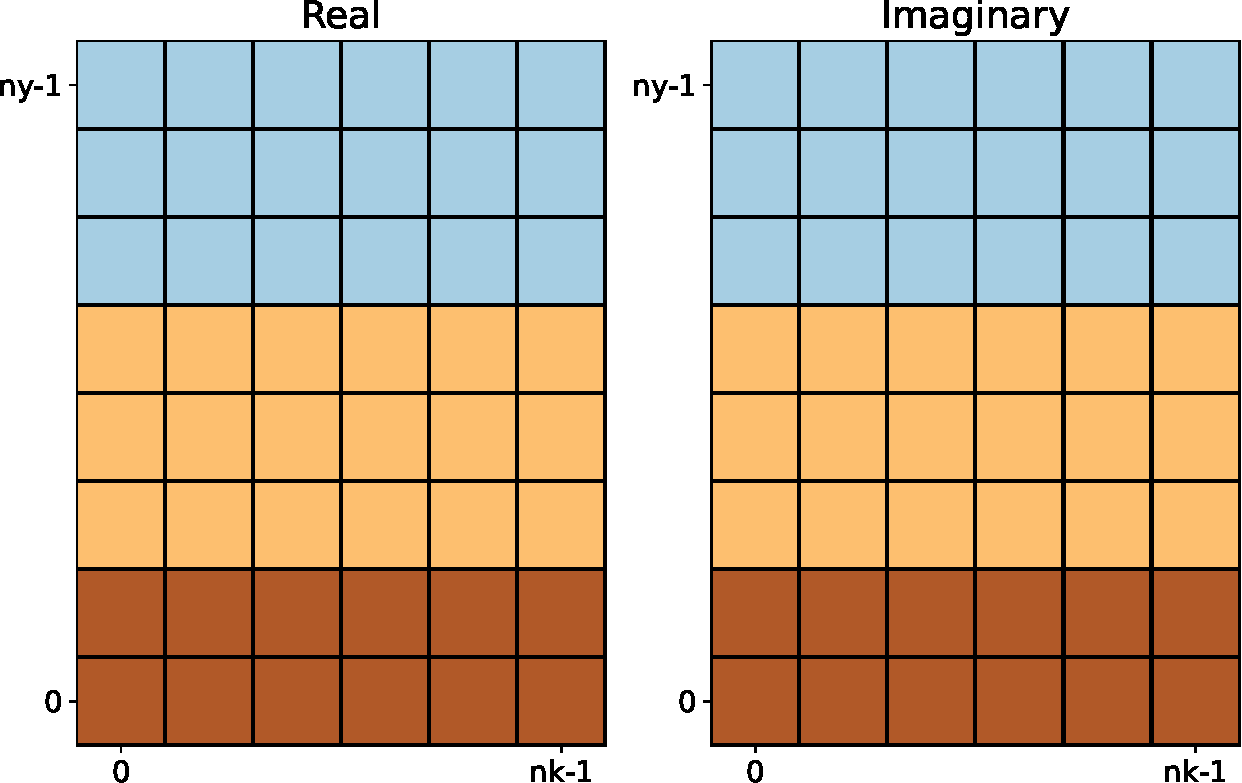
\includegraphics[width=0.6\textwidth]{step2.pdf}
\end{center}

The third step is a global communication (\texttt{MPI\_Alltoallv}) to make sure that each column is handled by a single task:

\begin{center}
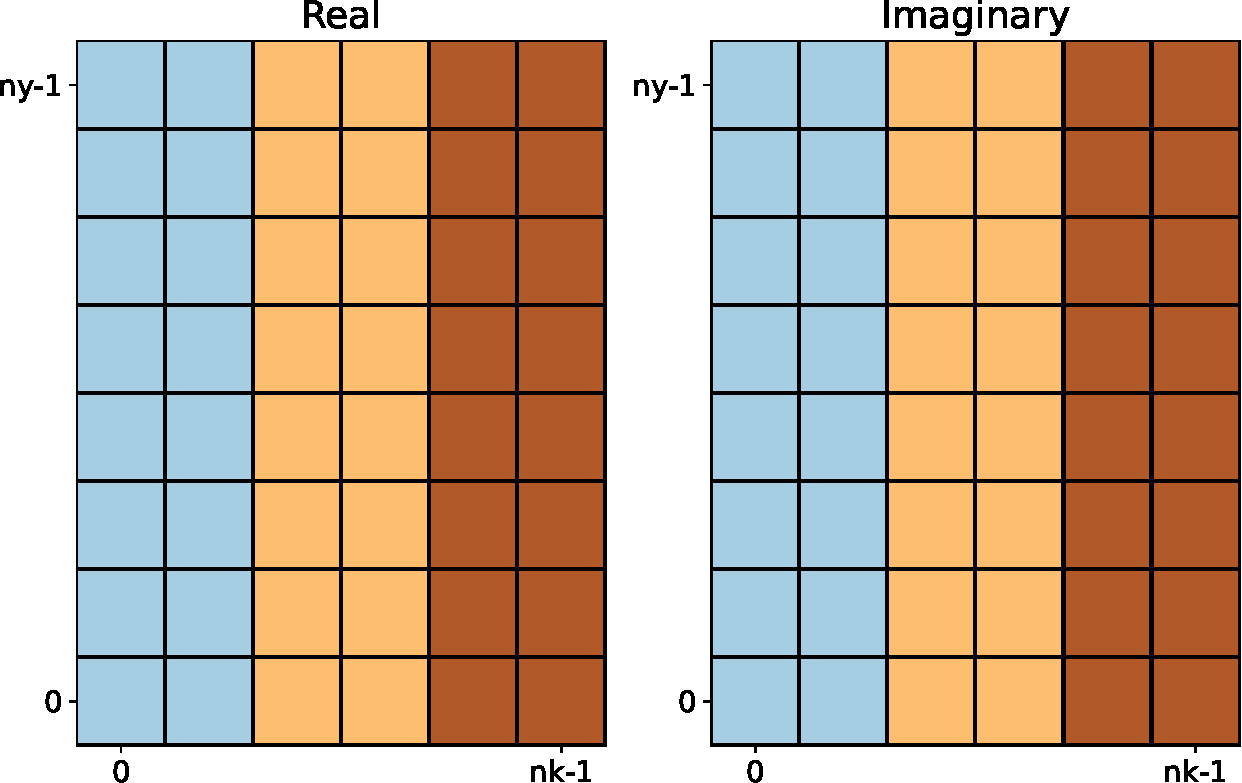
\includegraphics[width=0.6\textwidth]{step3.pdf}
\end{center}
   
The fourth step is a FFT along each column, leading to four arrays of size $n_k \times n_l$ for real/real, real/imaginary, imaginary/real and imaginary/imaginary components:
   
\begin{center}
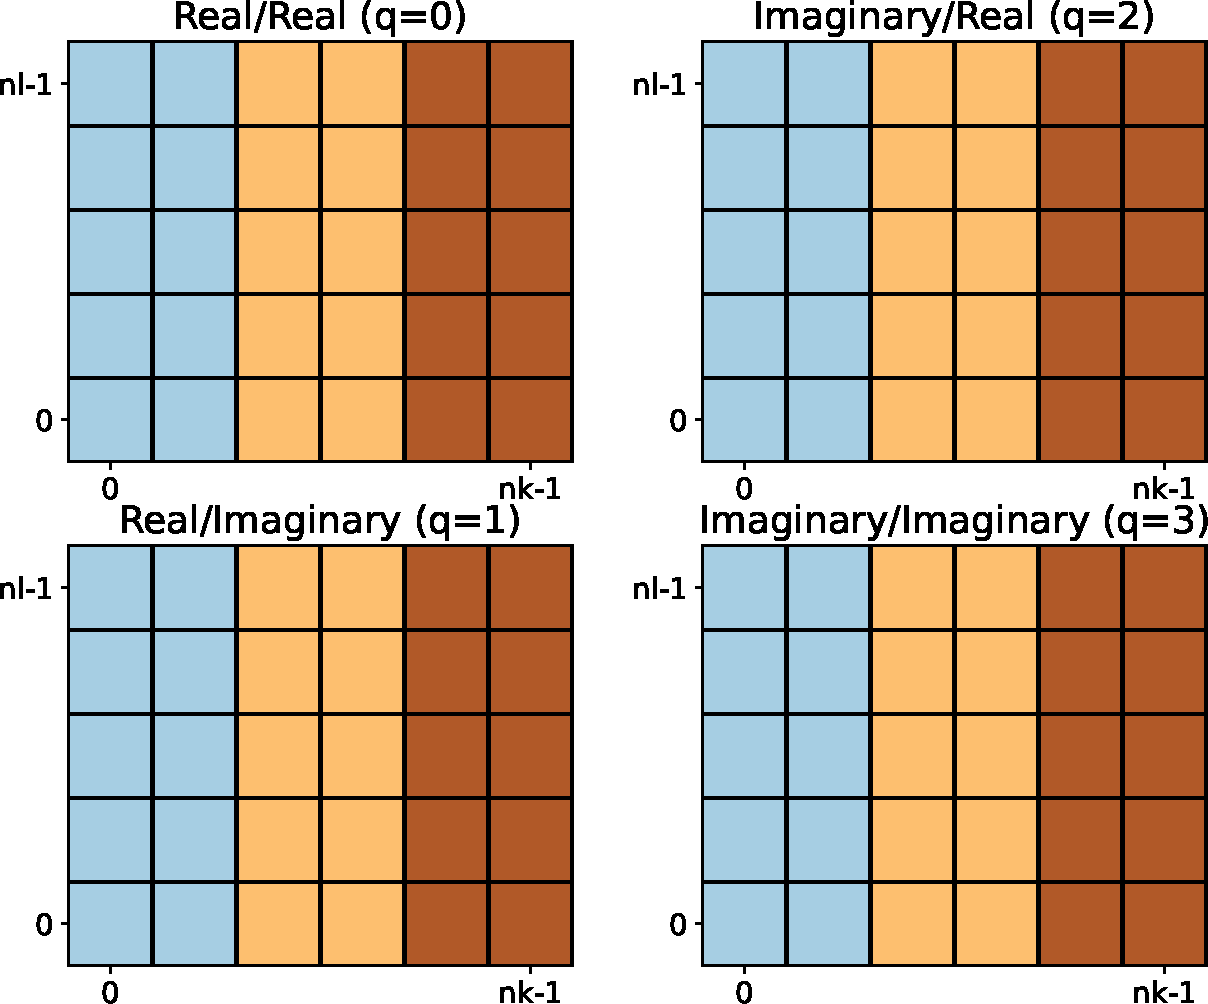
\includegraphics[width=0.6\textwidth]{step4.pdf}
\end{center}

The fifth step is the removal of redundant spectral coefficients because the input field is real. It is easy to check that the number of remaining spectral cofficients is exactly equal to the number of input grid points in physical space (same number of degrees of freedom):

\begin{center}
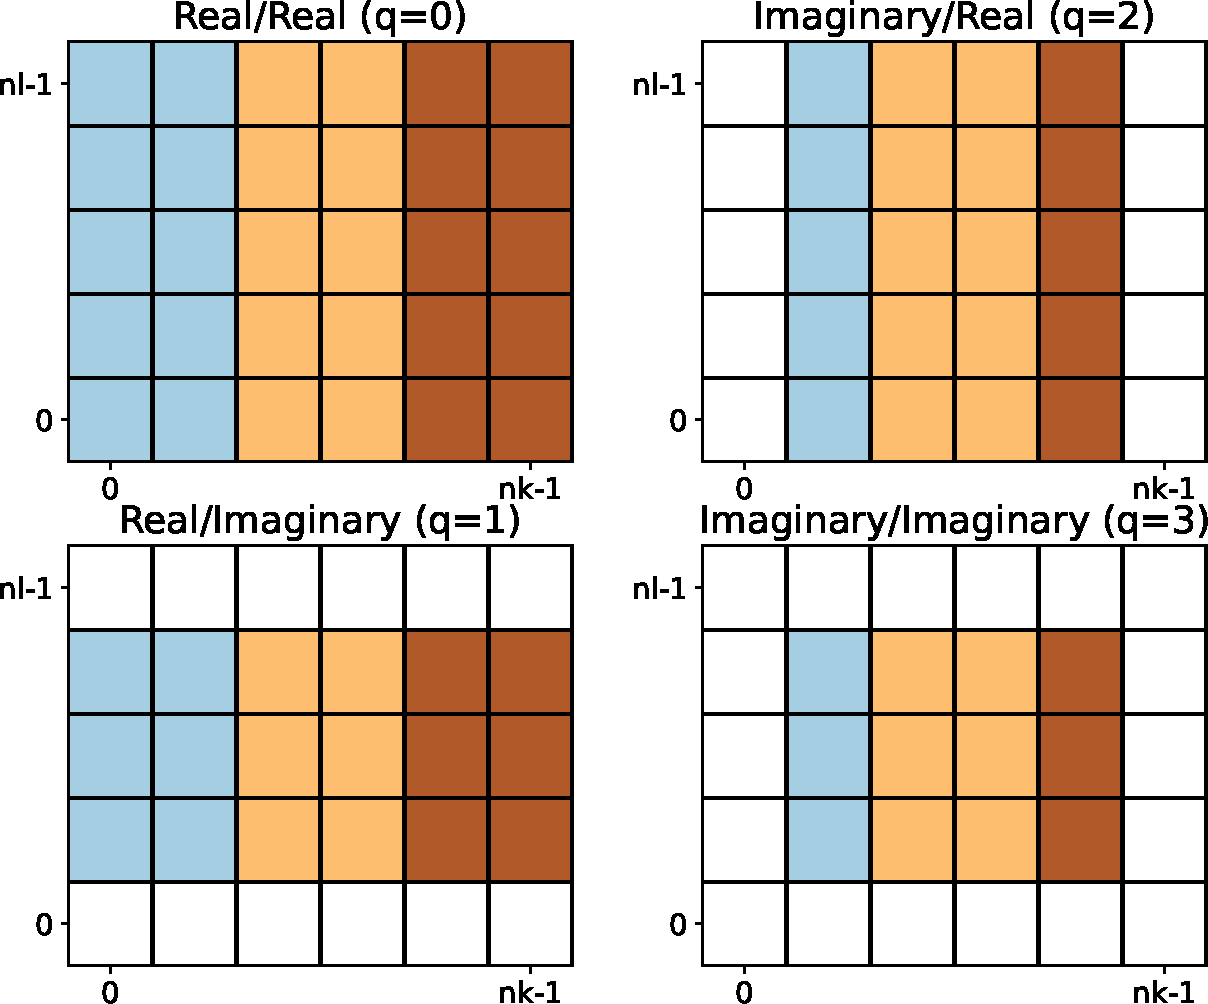
\includegraphics[width=0.6\textwidth]{step5.pdf}
\end{center}

The sixth step is an elliptic truncation on spectral wavenumber to ensure isotropy:
\begin{center}
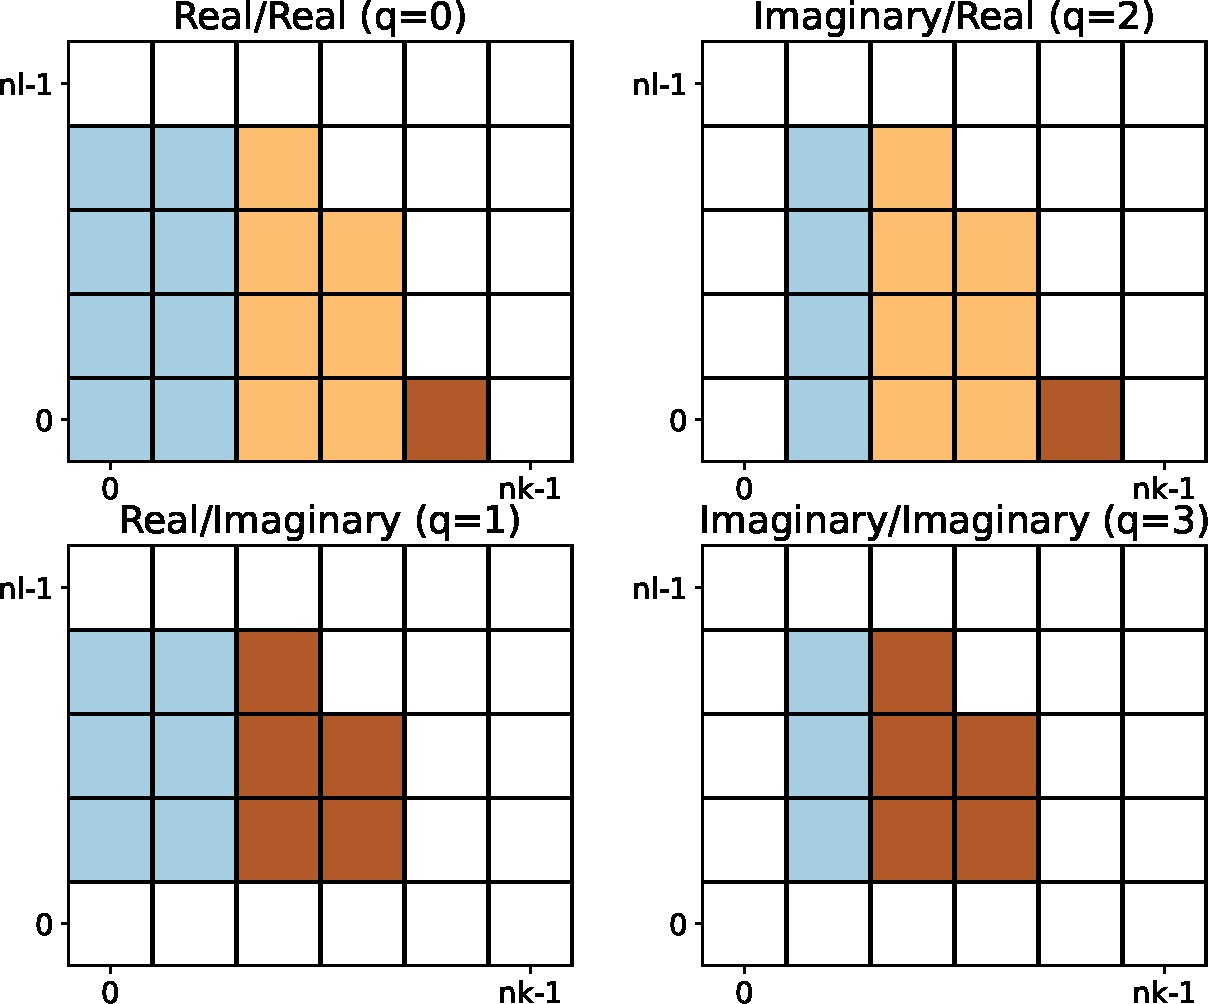
\includegraphics[width=0.6\textwidth]{step6.pdf}
\end{center}

The seventh step is a global communication (\texttt{MPI\_Alltoallv}) to split the remaining wavenumbers into equal chunks and improve the load balancing during calculations. It is important to keep all components of each couple $(k,l)$ on the same task to compute derivatives:

\begin{center}
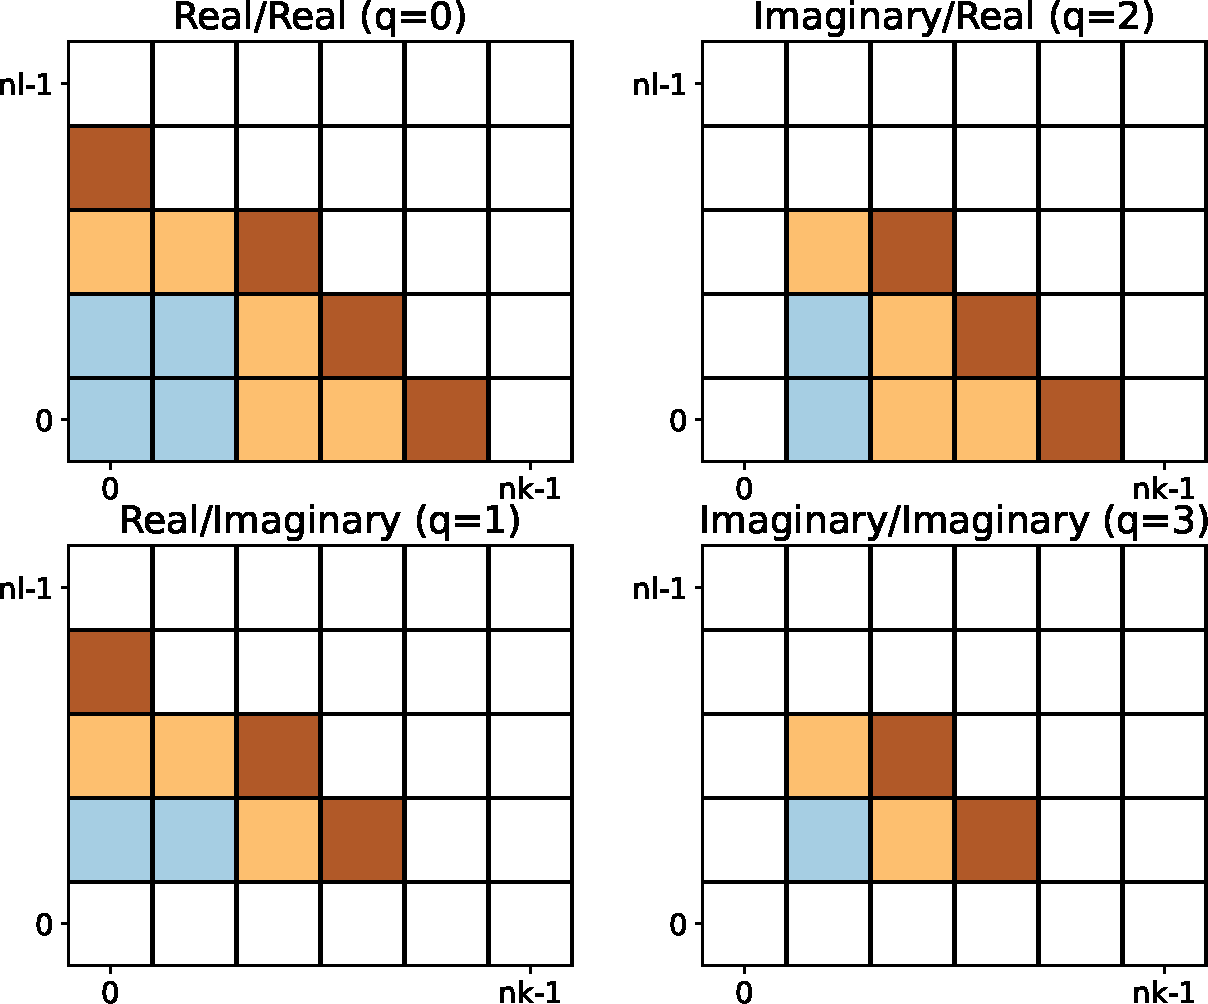
\includegraphics[width=0.6\textwidth]{step7.pdf}
\end{center}

Hereafter, we call "forward process" the sequence of these seven steps, and "inverse process" the backward sequence.

\subsection{Normalization}

The spectral transforms based on FFTW are not normalized, so a the spectral coefficient must be multiplied by $\sqrt{n_x n_y}$ at the end of the forward process, and at the beginning of the inverse process.

\subsection{Parseval's identity}

The Parseval's identity states that the canonical norm (i.e. squared canonical inner product of a field with itself) is the same in physical and spectral spaces. To verify the Parseval's identity with the decomposition described above, is is necessary to multiply each spectral coefficients at the end of the forward process by number of remaining component after the fifth step for its own $(k,l)$. For instance here:
\begin{itemize}
\item spectral coefficient for $(k,l) = (0,0)$ is multiplied by 1,
\item spectral coefficients for $(k,l) = (1,0)$ is multiplied by 2,
\item spectral coefficients for $(k,l) = (0,1)$ is multiplied by 2,
\item spectral coefficients for $(k,l) = (1,1)$ is multiplied by 4,
\item etc.
\end{itemize}

Of course, the input spectral coefficients must be divided by the same amount at the beginning of the inverse process. This operation has one major advantage: the adjoint of the forward process is now equivalent to the inverse process.

\section{Vorticity / divergence to physical wind}

\subsection{Derivatives}

In spectral space, computing derivatives is straightforward. Assuming that each spectral coefficient is defined by the triplet $(k,l,q)$:
\begin{itemize}
\item Derivative in X direction: $\mathbf{s}_\text{out} = \mathbf{D}_x \mathbf{s}_\text{in}$ with
\begin{subequations}
\begin{align}
\mathbf{s}_\text{out}(k,l,0) & = \frac{2 k \pi}{L_x} \ \mathbf{s}_\text{in}(k,l,2) \\
\mathbf{s}_\text{out}(k,l,1) & = \frac{2 k \pi}{L_x} \ \mathbf{s}_\text{in}(k,l,3) \\
\mathbf{s}_\text{out}(k,l,2) & = -\frac{2 k \pi}{L_x} \ \mathbf{s}_\text{in}(k,l,0) \\
\mathbf{s}_\text{out}(k,l,3) & = -\frac{2 k \pi}{L_x} \ \mathbf{s}_\text{in}(k,l,1)
\end{align}
\end{subequations}
where $L_x$ is the domain width in the X direction.
\item Derivative in Y direction: $\mathbf{s}_\text{out} = \mathbf{D}_y \mathbf{s}_\text{in}$ with
\begin{subequations}
\begin{align}
\mathbf{s}_\text{out}(k,l,0) & = \frac{2 l \pi}{L_y} \ \mathbf{s}_\text{in}(k,l,1) \\
\mathbf{s}_\text{out}(k,l,1) & = -\frac{2 l \pi}{L_y} \ \mathbf{s}_\text{in}(k,l,0) \\
\mathbf{s}_\text{out}(k,l,2) & = \frac{2 l \pi}{L_y} \ \mathbf{s}_\text{in}(k,l,3) \\
\mathbf{s}_\text{out}(k,l,3) & = -\frac{2 l \pi}{L_y} \ \mathbf{s}_\text{in}(k,l,2)
\end{align}
\end{subequations}
where $L_y$ is the domain width in the Y direction.
\end{itemize}
In both directions, $\mathbf{s}_\text{out}(k,l,q)$ is set to zero if the corresponding $\mathbf{s}_\text{in}$ component has been removed at step five of the forward process.

\subsection{Laplacian}

The Laplacian operator and its inverse are even simpler:
\begin{itemize}
\item Forward Laplacian: $\mathbf{s}_\text{out} = \mathbf{L} \mathbf{s}_\text{in}$ with
\begin{align}
\mathbf{s}_\text{out}(k,l,q) & = -\left(\frac{4 \pi^2 k^2}{L_x^2}+\frac{4 \pi^2 l^2}{L_y^2}\right) \ \mathbf{s}_\text{in}(k,l,q)
\end{align}
\item Inverse Laplacian: $\mathbf{s}_\text{out} = \mathbf{L}^{-1} \mathbf{s}_\text{in}$ with
\begin{align}
\mathbf{s}_\text{out}(k,l,q) & = -\frac{1}{\displaystyle \frac{4 \pi^2 k^2}{L_x^2}+\frac{4 \pi^2 l^2}{L_y^2}} \ \mathbf{s}_\text{in}(k,l,q)
\end{align}
and $\mathbf{s}_\text{out}(0,0,0) = 0$
\end{itemize}

\subsection{Wind variables}

We denote:
\begin{itemize}
\item $u$: zonal wind
\item $v$: meridional wind
\item $\psi$: stream function
\item $\chi$: velocity potential
\item $\zeta$: vorticity
\item $\delta$: divergence
\end{itemize}

Computing $(\zeta, \delta)$ from $(u, v)$ is straightforward:
\begin{subequations}
\begin{align}
\zeta & = \mathbf{D}_x v - \mathbf{D}_y u \\
\delta & = \mathbf{D}_x u + \mathbf{D}_y v
\end{align}
\end{subequations}

The inverse operations requires two steps:
\begin{subequations}
\begin{align}
\psi & = \mathbf{L}^{-1} \zeta \\
\chi & = \mathbf{L}^{-1} \delta
\end{align}
\end{subequations}
and
\begin{subequations}
\begin{align}
u & = \mathbf{D}_x \chi - \mathbf{D}_y \psi \\
v & = \mathbf{D}_x \psi + \mathbf{D}_y \chi
\end{align}
\end{subequations}

\section{Balance operator}

\section{Covariance operator}


\bibliographystyle{mybib-en}
\bibliography{bifourier}
\end{document}
